\chapter{Pipeline parallelism for Javascript} \label{chapter4}

%\chapter{A framework for parallel web applications}
 % \section{Fluxions}

% \chapter{Fluxion}

%   \section{Fluxionnal Compiler}
%     \comment{Some parts of this are already written in the first paper. It needs a lot additional explanations and rewritting}
%     \subsection{Identification}
%       \subsubsection{Continuation and listeners}
%       \subsubsection{Dues}
%     \subsection{Isolation}
%       \subsubsection{Scope identification}
%         \comment{Scope leaking}
%       \subsubsection{Execution and variable propagation}
%     \subsection{distribution}

%   \section{Fluxionnal execution model}
%     \comment{Everything here is already written in the first paper  : flx-paper. It only needs to be rewritten}
%     \subsection{Fluxion encapsulation}
%       \subsubsection{Execution}
%       \subsubsection{Name}
%       \subsubsection{Memory}
%     \subsection{Messaging system}

% \chapter{Evaluation}
%   \section{Due compiler}
%   \section{Fluxionnal compiler}
%   \section{Fluxionnal execution model}


The conclusion of the state of the art is that no platform allows to follow a project from the early beginning to the maturation of the project.
Indeed, no platform can provide alternatively productivity and efficiency.
All the platform tends to focus on a static compromise between these two goals, and therefore, are useful only at a precise point in the project.
They either grow useless, or are too complicated to begin with.

This chapter presents the solution developped in this thesis.
A platform to follow web application projects from the early beginning until the maturation of the project.

To support this evolution, it support a continuous developpement.

\section{Seamless Development} \label{chapter3:objectives}
\nt{TODO title not clear enough}

\begin{center}
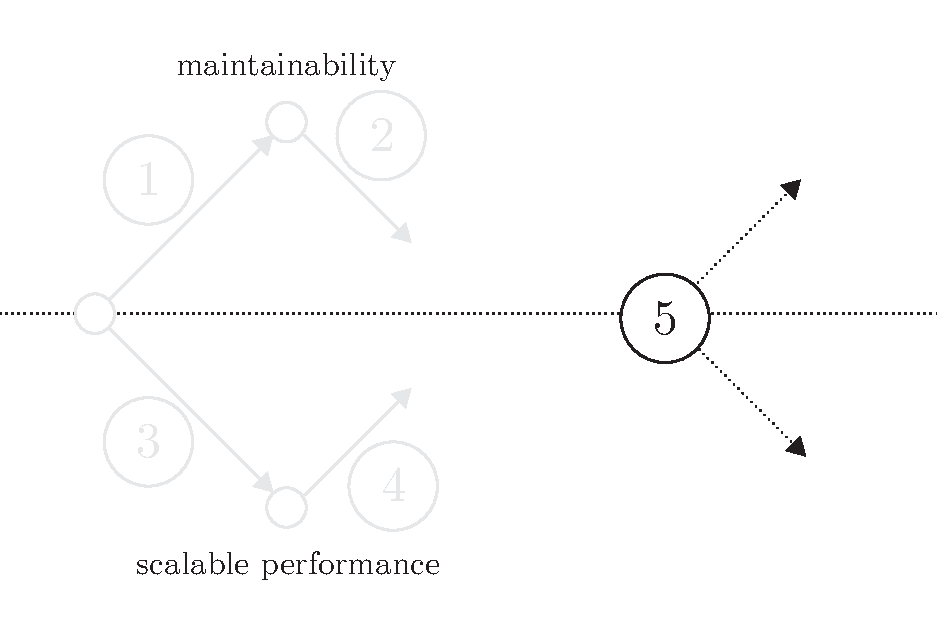
\includegraphics[width=0.6\textwidth]{../ressources/state-of-the-art-5.pdf}
\end{center}

The section \ref{chapter3:software-maintainability} shows that the modular organization enabled by functional programming is the best way to improve maintainability.
But it requires the use of a global memory store which conflicts with performance.
Compilation is a solution to reduce this conflict, but is not yet satisfactory enough for high performance scalability.
On the other hand, the section \ref{chapter3:software-performance} shows that to attain performance scalability, an application needs to multiply the exclusive accesses to its state.
That implies follow a distributed organization of its state to provide isolation and immutability, which negatively impacts modularity, hence maintainability.
Some works provide a uniform memory access to improve maintainability, despite the distributed execution.

The evolution of the economical constraints of a web application requires to repeatedly switch between maintainability and performance scalability.
The incompatibility between the two organizations implies technological ruptures at each switch.
Huge developing efforts are pulled to translate manually from one organization into the other, and later to maintain the implementation despites its unmaintainable nature.
There is still room for improvements on a compromise between maintainability and performance scalability.

The state of the art highlighted that
\begin{itemize}
\item maintainability requires lazy-evaluation and higher-order programming, section \ref{chapter3:software-maintainability:programming-models:functional-programming}, and
\item higher-order programming requires a global memory abstraction, section \ref{chapter3:software-maintainability:modular-programming:limitations},
\end{itemize}
Javascript is a functional language that features higher-order programming and a global memory abstraction.
% Moreover, its dynamic natures allows a lot of flexibility for the developers.
Moreover, node.js features a streaming approach with the event-loop execution model, similar to the lazy evaluation.
These reasons make Javascript a language of choice for developing web application.

And that
\begin{itemize}
\item scalable performance requires parallelism, and
\item parallelism requires exclusive accesses on the state through isolation and immutability.
\end{itemize}
Eventually, web development is heading toward a streaming approach with pipeline processing.

\nt{TODO dependency schema of these highlights}

This thesis proposes an equivalence between the global memory and control flow on one hand, and memory isolation with message passing on the other hand.
It proposes this equivalence as a solution to conciliate the scalable performance and maintainability.
As explained below, the concurrency model of the event-loop execution model, and the parallel approach of the pipeline execution model are very similar.
The goal of this thesis is to allow to compile one execution model into the other, to allow developers to constantly keep two organization of their implementation, allowing them to focus on both maintainability and scalable performance.

\subsection{Equivalence}

The next paragraphs introduces this equivalence between the event-loop execution model and the pipeline execution model.
The equivalence addresses two \textit{levels}\nt{not the good word}, as illustrated in figure \ref{fig:chapter3:objectives:roadmap}, the control flow, and the memory isolation.

\begin{figure}[h!]
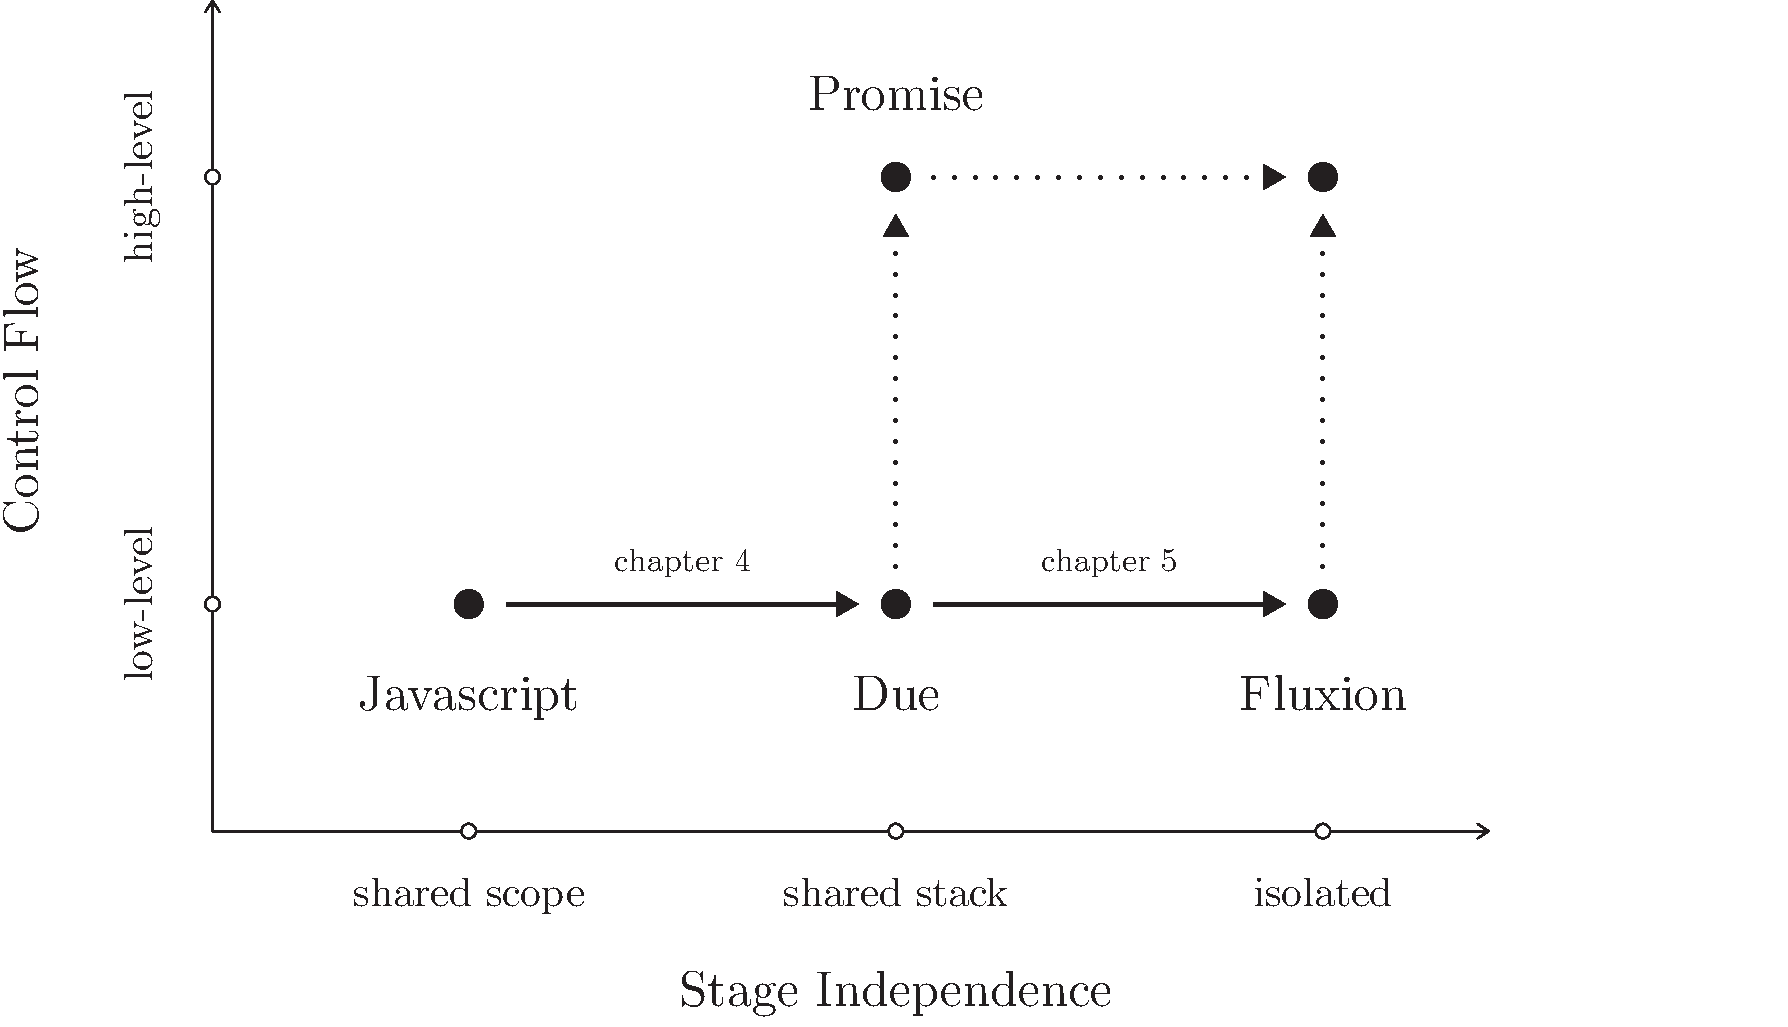
\includegraphics[width=1\textwidth]{../ressources/roadmap.pdf}
\caption{Roadmap}
\label{fig:chapter3:objectives:roadmap}
\end{figure}

\subsubsection{Rupture Point}

The execution of the pipeline architecture is well delimited in isolated stages.
Each stage has its own thread of execution, and is independent from the others.
On the contrary, the code of the event-loop is linear because of the continuation passing style and the common memory store.
% The message passing linking the callbacks is transparently handled by the event-loop.
However, the execution of the different callbacks are as distinct as the execution of the different stages of a pipeline.
The call stacks of two callbacks are distinct.
Therefore, an asynchronous function call represents the rupture between two call stacks.
It is a rupture point, and is equivalent to a data stream between two stages in the pipeline architecture.

Both the pipeline architecture and the event-loop present these rupture points.
The detection of rupture points allows to map a pipeline architecture onto the implementation following the event-loop model.
To allow the transformation from one to the other, this thesis studies the possibility to detect rupture points, and to distribute the global memory into the parts defined by these rupture points.
The detection of rupture points is addressed in chapter \ref{chapter4}.

It presents the extraction of a pipeline of operations from a Javascript application.
Indeed, such pipeline is similar to the one exposed by Promises.
The chapter proposes a simpler alternative to the latter called Dues.
However, these operations still require a global memory for coordination so they are not executed in parallel.

\subsubsection{Invariance}

% This transformation is important on two points.
% The conservation of the invariance.
% The equivalence between the coordinations.

The transformation should preserve the invariance as expressed by the developer to assure the correctness of the execution.
The partial ordering of events in a system, by opposition to total ordering, is sufficient to assure this correctness.
% This result was used by Lamport to prove the correctness of distributed systems.
The global memory is a way to assure the total ordering of events, and the message passing coordination is a way to assure partial ordering of events.
Therefore, to assure the correctness of the execution of a system, the state coordination with a global memory is equivalent to message passing coordination.
And it is possible, at least for some rupture points, to transform the global memory coordination into message passing while conserving the correctness of execution.

In order to preserve the invariance assured by the event-loop model after the transformation, each stage of the pipeline needs to have an exclusive access to memory.
The global memory needs not to be split into parts and distributed into each of the stages.
To assure the missing coordinations assured by the shared memory between the stages, the transformation should provide equivalent coordination with message passing.
The isolation and replacement of the global memory is fully address in chapter \ref{chapter5}, with the introduction of isolated containers called Fluxions.




% The invariance holds for the whole memory during the execution of each callback.
% As I explained in the previous section, this invariance is required to allow the concurrent execution of the different tasks.
% On the other hand, the invariance is explicit in the pipeline architecture, as all the stages have isolated memories.
% The coordination between these isolated process is made explicit by the developer through message passing.

% I argue that the state coordination between the callbacks requireing a global memory could be replaced by the message passing coordination used manually in the pipeline architecture.
% I argue that not all applications need concurrent access on the state, and therefore, need a shared memory.
% % Specifically, I argue that each state region remains roughly local to a stage during its modification.
% \nt{TODO review that, I don't know how to formulate these paragraphs. Identify the state and the data in the global memory.}

% \subsubsection{Transformation}

% This equivalence should allow the transformation of an event loop into several parallel processes communicating by messages.
% In this thesis, I study the static transformation of a program, but the equivalence should also hold for a dynamic transformation.
% I present the analyzis tools I developed to identify the state and the data from the global memory.

% % # Explanation of the concept

% ## Turn-based programming.

% (see presentation on Dues)
% -> single-thread, no wait, no block and so on
% Shared heap -> no mutex, no synchronization, so it is good scalability


% Turn-based programming is an event-loop.
% It is the execution of queued events one after the other.
% An event is the association of a callback and a message.
% The callback is a small Javascript Program, designed to process the message.
% During its turn, the callback executes, and can queue events : that is register callback to be executed during a next turn.
% TODO what I mean exactly by queue events ? -> the distinction between the asynchronous operation, and the resulting event.

% ## Pipeline

% So a callback sends messages to other callbacks.
% -> It is exactly like a pipeline.
% However, all the callbacks share the same heap.
% So it is not possible to distribute the different callbacks without synchronization of this heap, or splitting the heap for each callback.
% TODO state VERY clearly this problem, it is at the core of my thesis.

% So, how to split the heap so that each callback has its own exclusive heap ?

\comment{From here, the reader should be confortable with the event-loop, and the analogy we drawn between the event-loop and a pipeline.
The problematic is now clear : how to split the heap so that each asynchronous callback has its own exclusive heap ?}

\section{Callback identification}

\subsection{\comment{TODO}}

\section{Callback isolation}

We explain in this section the compilation process we developped to isolate the memory access for each callbacks.
The result of this process should be two-fold. First each callback should have an exclusive access on a region of the memory. So that two different callback can be executed in parallel. And it should be clear for each callback, what are the variable needed from upstream callbacks, and what are the variable to send downstream.

\subsection{Propagation of variables}


\subsubsection{Scope identification}

In section \ref{??? Javascript scope / closure}, we explained that Javascript is roughly lexically scoped.
A consequence is that the declaration of contexts can be inferred statically.
For example, in a lexically scoped, strongly typed, compiled language, the compiler know the content of each scope during compile time, and can prepare the memory stack to store the variables in each scope.

In most languages, the memory is in two parts : the stack, and the heap.
The stack is statically scoped, and its layout is known at compile time.
The heap, on the other hand is dynamically allocated. Its layout is built at run time.

But Javascript is a dynamic language, perhaps the most dynamic of all languages.
It doesn't have this distinction between stack and heap. Every variable is dynamically allocated on the heap.
That induce two consequences.
The first is that Javascript provides two statements to dynamically modify the lexial scope : \texttt{eval} and \texttt{with}.
The second is that to know the layout of the heap, we need to use static analysis tools.
In the next two sections, we adress these two consequences.

\subsubsection{Break the lexical scope} \label{???:breakscope}

Without these statements, \texttt{eval} and \texttt{with}, Javascript is lexically scoped. It is possible to infer the scope of each variable at compile time.


The \texttt{with} statement continue the execution using an expression as the lexical scope.
As the provided expression is dynamically evaluated, it is possible to dynamically modify the lexical scope.
The code snippet below show an example of such a situation.

\begin{code}
var aliveCat = {isAlive: true};
var deadCat = {isDead: true}

with (Math.random() > 0.5 ? aliveCat : deadCat) {
  isAlive;
  // Half the time -> ReferenceError: isAlive is not defined
  // Half the time -> true;
}
\end{code}

The variable \texttt{isAlive} is defined only in the object \texttt{aliveCat}.
The presence of the variable \texttt{isAlive} in the lexical environment within the \texttt{with} statement cannot be determined statically, as the lexical environment is dynamically linked to either \texttt{aliveCat} or \texttt{deadCat}.

Note that the MDN reference page on \texttt{with}\ftnt{https://developer.mozilla.org/en-US/docs/Web/JavaScript/Reference/Statements/with} says that \textit{Using \texttt{with} is not recommended, and is forbidden in ECMAScript 5 strict mode.}

The \texttt{}

% TODO and specify that Javascript is roughly lexically scoped : it is not completely lexically scoped, and five examples to backup that.

Not to be mistaken with the \texttt{this} operator.
It is possible to dynamically change the content of an object,  
% TODO continue this paragraph about how the this operator change the properties of an object. 
% Does it change the lexical scope, if that object is actually used as a context elsewhere ? -> No, I don't think so.
% But ask on SO, just to be sure.

\begin{code}
function stuff() {
  this.x = 42;
}

stuff.call({})

\end{code}

% Javascript is lexically scoped, therefore we can identify the the scope of variable statically.
% (At the exception of eval and with : with is forbidden from strict mode, so that is not a bigdeal, howether, eval is sometimes used in smart ways, but most of the time it is monomorphic (I don't exactly know what that means, I heard from Floreat, it must be something related to PL community)).

% The compiler identifies the variables shared by multiple callbacks from their scope.
% TODO explain this in depth.
% Function scope, closures, and so on ...



However, even if Javascript is lexically scoped, the memory is still dynamicall allocated and manipualeted, so that it is not possible to actually infer the memory layout at compiler time only with lexical scope analysis, and without deeper static analysis.

\subsubsection{Scope Leaking}

% Javascript uses a pass-by-sharing paradigm.
% That means that sometimes the argument of a call are passed by value, sometimes by reference (atomic data type (number, string, bool) -> by value, complex data type (objects) -> by reference).
% That means that the modification of a local variable can affect variable in seemingly unrelated scopes.
% It seems that the points-to analysis is what is used to find stuffs like that (side-effects ?).

% TODO what we are talking about here are aliases.

% TODO I am stating here that in low-level language, the memory access is so fine, that it is difficult to exactly pin down the memory layout in term of object, it is rather seen as a big array of memory adresses.
% While in higher-level language, like Javascript, the memory access is at the property level (it is not possible to access memory down to the adress), so it could be easier (maybe, just not harder) to infer the dynamic memory layout from source.
To infer the layout of the heap at compile time, static analysis tools are used, like the points-to analysis, developped by Andersen in its PhD thesis \cite{Andersen1994}.
For such analysis, the memory is splitted at the access scale.
In low-level languages, like C/C++, the memory is mainly managed by the developer. Allowing access to the memory at a small grained scale : up to the address.
It impose the analysis to split the memory to the adress scale in some cases.
% TODO Backup that, HEAVILY
In higher-level languages, like Javascript, the developer cannot access the memory to the adress scale.
The memory is accessed at a coarser scale : the property scale.
(At the exception of some arrays and buffers, that mimic, and are mapped to actual memory adresses for performance reasons.)
% TODO find exactly the references for these buffers : I think of ArrayBuffer, and sharedArray ... but I am not sure. Need more inspection.

\subsubsection{Propagation of execution and variables}

For the execution of each callback / stage, the corresponding part of the state is local, and the rest is remote, and inaccessible.
We are going to explain why it must remain inaccessible.

While a callback is executing a request, the previous callback (the up stream callback) is executing the next request.
The next request will arrive at the current callback some time in the future.
The modification done in the state of the upstream callback will propagate only later in the current callback.
The state of the upstream callback is in a different time frame than the state of the current callback.

To really understand that, we need to compare this execution with the execution on a unique event-loop.
If the current callback executes, then the upstream callback might have, or might not have started to execute the next request.
But as soon as the current callback executes, the modifications done on the states, are immediatly propagated, so that the upstream callback can take them into account for the next request.

However, if the two callbacks are distant, then the modification of the current callback will not immediatly propagate to the upstream callback.
During the propagation, the upstream callback might execute requests than would not be aware of the state modification from the current callback (from downstream).
That is why we say the upstream callback and the current callback are in two different time frame.
Propagating the state modification upstream is like going backward in time, it is impossible.
That is why the execution, and the state modification propagation must always flow downstream.

As a note, I must add that if an upstream and a downstream callbacks are on the same event-loop, then this doesn't apply. it is like a loop in the time : the modification immediatly propagate from downstream to upstream.






% The execution progress downstream, following the message stream.
% TODO state very clearly this proposition, it is the second core of my thesis (and I love the idea, it relates directly to reality, graivity, and the fabric of the universe <3).

% Because the propagation of the modification is not instantaneous, going back upstream is like going backward in time : it is impossible.
% Therefore, a variable cannot be read upstream a write.
% And it cannot be write downstream either.

% In other words, only one callback can write on a variable -> seems obvious from previous sections.


% In promises, because the heap is not shared, things are less restrictive.
% Multiple stages can read and write the same variable, because the propagation of modification is instantaneous, due to the shared heap.





% TODO write about what it implies to detect continuation in variable, or other expressions.

% Why can we only detect continuations declared in situ.
% If a continuation is passed as a variable, we don't know for sure what is the function associated with, and the closure of that function.
